\documentclass[preprint,12pt,nopreprintline]{elsarticle}
\usepackage[T1]{fontenc}
\usepackage{lmodern,microtype,graphicx,booktabs,amsmath,amssymb,array,tabularx,longtable,xurl}
\usepackage[hypertexnames=false]{hyperref}
\setlength{\emergencystretch}{2em}
\renewcommand{\topfraction}{0.9}
\renewcommand{\bottomfraction}{0.8}
\renewcommand{\textfraction}{0.08}
\renewcommand{\floatpagefraction}{0.55}
\hypersetup{hidelinks,pdfauthor={Author-review draft},pdftitle={Reference-Preserving Speculative Decoding on Consumer Systems},pdfsubject={JSA v0.14.0 author-review manuscript; not submitted}}
\newcommand{\RQtag}[1]{\textbf{RQ#1}}
\makeatletter
\def\ps@pprintTitle{\let\@oddhead\@empty\let\@evenhead\@empty\def\@oddfoot{\hfil\thepage\hfil}\let\@evenfoot\@oddfoot}
\makeatother
\begin{document}
\begin{frontmatter}
\title{Reference-Preserving Speculative Decoding on Consumer Systems: Diagnosis, Repair Scope, and Paid Cost}
\author{Author information pending confirmation}
\begin{abstract}
Speculative decoding can change a quantized runtime's greedy output as well as its cost. When a fixed ordinary output must be reproduced, a runtime designer must decide where to constrain execution and whether the qualified transformation pays. We study these decisions through retained-state interventions, a phase-scoped attention implementation, and paid ordinary and matched draft-free comparisons. Natural state--current-recipe crosses reveal path effects and interactions on CUDA and Vulkan. A same-state single-block intervention changes downstream trajectories despite unchanged immediate decisions. On RTX, mapping attention queries into the batch dimension preserves other batched computation; target prefill and continuation are inclusion-minimal within a tested four-switch family. A frozen recipe qualifies full responses on 24 project-unused inputs. Generation speed is 1.170 times ordinary and 1.169 times matched decoding. Resident-request speed is 1.742 times ordinary but 1.035 times matched: the draft-free target-path change already provides 1.683 times. Seven tasks regress against matched request cost, and one round reverses direction. Wider fixed-capacity drafting and a B570 endpoint repair qualify while losing performance. Historical M4 and 358H results limit the case for added control and draft-only optimization. The contribution is a concrete runtime design study linking local diagnosis, finite repair qualification, and paid cost, with failure boundaries retained. Repair evidence remains specific to the tested Qwen3 implementation family and configurations.
\end{abstract}
\begin{keyword}
speculative decoding \sep numerical consistency \sep execution state \sep runtime design \sep performance evaluation \sep consumer systems
\end{keyword}
\end{frontmatter}
\section{Introduction}
\label{sec:introduction}
Speculative decoding accelerates autoregressive inference by proposing tokens with a draft and evaluating several positions with the target~\cite{leviathan2023}. Its appeal on consumer systems is practical: additional intra-request work can amortize target execution when memory and traffic do not permit large inter-request batches. Yet replacing scalar continuation with speculative execution changes numerical call shapes, retained state, and bookkeeping. A mathematically valid sampling rule does not by itself certify that a particular quantized implementation reproduces a selected greedy output or lowers the cost of doing so.

We consider systems in which an ordinary greedy execution defines the required reference. Examples include regression testing and repeatable application behavior under a registered runtime configuration. The requirement is token or endpoint equality to that execution, rather than a claim that its answer is functionally correct or that every floating-point value is identical. This makes two engineering decisions inseparable. The designer must determine where execution consistency needs to be enforced, then measure whether the qualified transformation is useful. Constraining the wrong boundary can repair one input and introduce another deviation. Constraining all computation can recover output while losing the intended acceleration.

The boundary is not determined by the visible token prefix alone. Two executions can have emitted the same tokens while retaining different numerical key/value (KV) contents or pending state. Their next decision can depend on that history, on the current execution recipe, or on an interaction between them. Conversely, changing a score need not change the immediate greedy decision. An unchanged decision at one verification block can still precede different downstream output. These distinctions determine whether an implementation needs to constrain state formation, current continuation, or both.

The cost comparison has a related ambiguity. A repair can improve the target path before any drafting occurs. Comparing only repaired speculation with the ordinary reference assigns that path benefit to the entire deployment change. It does not isolate the value of speculation. A matched target-only path, using the repaired target execution without a draft, is therefore a second paid comparator. Neither comparator can be replaced by accepted-token fraction, target-call count, or isolated draft throughput.

Our cases show why both decisions matter. An RTX continuation intervention repairs one task and regresses another while preserving aggregate reference agreement. A later phase-scoped attention implementation qualifies full responses on 24 inputs unused in the accessible project history. Its resident-request speed is $1.742\times$ ordinary decoding, but matched draft-free execution already gives $1.683\times$; speculation adds $1.035\times$ on that path. A separate B570 implementation preserves the registered endpoint yet is substantially slower than both paid draft-free comparators. These outcomes support a system design study built around three questions:
\begin{enumerate}
\item \RQtag{1}, diagnosis: does a deviation follow retained numerical state, the current recipe, or their interaction?
\item \RQtag{2}, repair: within a defined implementation family, which phase constraints are sufficient to preserve the reference?
\item \RQtag{3}, cost: when qualification holds, what benefit remains against ordinary decoding and against a matched target path?
\end{enumerate}

The contributions are concrete. First, controlled natural-state crosses with own-path shams expose different local dependencies on CUDA and Vulkan; a separate B570 single-block intervention shows why immediate agreement cannot replace trajectory qualification. Second, an RTX query-layout transformation preserves batched projection and feed-forward work, with a four-switch factorial locating a sufficient target-phase scope in the tested family. Third, ordinary/matched/candidate costs and qualified counterexamples change the engineering decision about adding speculation, increasing draft width, retaining a guard, or optimizing only the draft.

Numerical path sensitivity, consistent KV state, fixed-shape verification, and verification overhead have established research foundations. We do not claim their discovery or a new general sampling algorithm. The additional contribution is the implemented constraint, controlled evidence about its scope, and the consequences for measured operating choices. The diagnosis is an offline experimental procedure, not a validated automatic online selector. The target models belong to one Qwen3 family; four hardware cases do not substitute for cross-family repair evidence.

Sections~\ref{sec:runtime} and~\ref{sec:methods} define the runtime and contracts. Sections~\ref{sec:diagnosis}--\ref{sec:cost} answer the three questions. Section~\ref{sec:implications} states the resulting design decisions and limits. Supplementary material S1 gives campaign-level details, historical results, failures, and missingness; S2 is the author source and arithmetic-reproduction bundle.

\section{Runtime Architecture and Research Context}
\label{sec:runtime}
\subsection{Execution as a stateful transaction}
A speculative iteration advances a committed prefix through draft, target verification, and reconciliation. The draft proposes up to $k$ tokens. The target evaluates the pending token and proposal positions, often through a caller batch containing several tokens. Acceptance, correction, and a possible bonus token determine what is committed. Rejected positions must then be removed or reconciled before the next iteration. Stopping is evaluated under the registered EOG and cap rule. Figure~\ref{fig:architecture} locates the state interfaces and the four phase controls examined here.

The runtime state includes more than committed IDs. Target and draft KV ownership, logical positions, pending logits or tokens, sampler history, and loop counters connect successive calls. A pending token may already have been sampled and accepted into the sampler while remaining to be evaluated into the cache. A transfer that repeats or omits this event changes the transaction. Early intervention frontends therefore retain pending state and clone behavior as well as KV. The later B570 candidate instead binds phases in the same context and live sampler. The RTX cost candidate does not activate its optional state-transplant branch.

\begin{figure}[!htbp]
\centering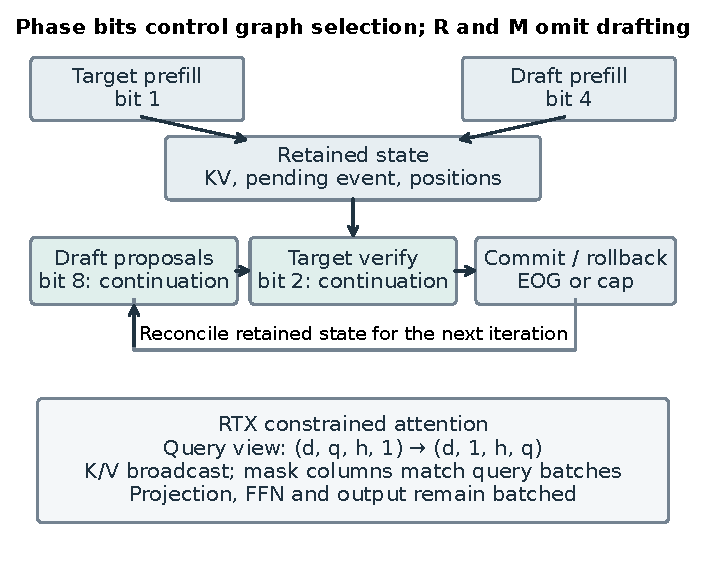
\includegraphics[width=\linewidth]{figures/figure_1_architecture.pdf}
\caption{Execution transaction and consistency controls. Bits 1/2 constrain target prefill/continuation; bits 4/8 constrain draft prefill/continuation. Verification consumes retained target state and online proposals; commit/rollback reconciles the next iteration. $R$ and $M$ omit the draft loop. The diagram was prepared with ChatGPT/Codex-assisted plotting code from the source-bound interfaces; it does not imply that the RTX cost candidate performs state transplantation.}
\label{fig:architecture}
\end{figure}

The microbatch capacity, denoted UB, limits how a caller batch is partitioned for backend execution. It is distinct from $k$, occupied query count, and the number of output rows reserved by the frontend. UB2 can process a caller with one occupied continuation token. A larger $k$ can lower caller count while increasing the number of micrographs. Output reservation can change the recipe even at the same UB. These distinctions matter when interpreting a cross or a performance counter.

The native implementation is based on pinned llama.cpp releases and source-bound private frontends~\cite{llamacpp}. The late RTX graph uses Qwen3-8B as target and Qwen3-0.6B as draft~\cite{qwen3}, both Q8\_0, with non-flash CUDA attention. The intervention uses existing ggml views and operations; it adds neither a new CUDA arithmetic kernel nor a new acceptance rule. B570 uses Vulkan with a different frontend and phase-binding operation. Metal and OpenVINO-related historical cases retain their own runtime contracts. These are software execution choices on consumer hardware, rather than controlled comparisons of hardware alone.

\subsection{Reference preservation and prior determinism work}
The output requirement is deliberately narrower than general determinism. A token sequence can match while logits or cache values differ. Conversely, deterministic repetition of a candidate can stably reproduce the wrong reference. We register the ordinary path and endpoint before asking whether a transformation preserves them. Numerical consistency research already explains why shape-dependent reductions can alter such behavior. Batch-invariant inference constrains reduction strategies across batches~\cite{thinkingmachines}.

LLM-42 uses a decode--verify--rollback design, fixed verification shapes with padding, and replacement of decoded KV entries by verifier entries~\cite{llm42}. It also permits distinct consistent strategies for prefill and decode. Stage-Replay studies fixed-prefix precision controls and bidirectional cache transplantation~\cite{stagereplay}. Vosti specifies and verifies deterministic inference at a system level~\cite{vosti}. MarginGate uses margin-triggered verification and repairs confirmed mismatches~\cite{margingate}. These works establish principles that this manuscript uses rather than renames. Table~\ref{tab:related} states the specific additional evidence and the comparisons not performed.

\begin{table}[t]\centering\small
\caption{Closest research context and the scope of this study. No row implies an implementation or speed advantage over the cited method.}
\label{tab:related}
\begin{tabularx}{\linewidth}{@{}p{.23\linewidth}XX@{}}\toprule
Prior work & Established basis & Additional evidence here\\\midrule
Batch-invariant inference; LLM-42~\cite{thinkingmachines,llm42} & Reduction/shape consistency; verified tokens and KV reconciliation & Qwen3 query views, phase dispatch and finite scope, followed by ordinary and matched paid costs\\
Stage-Replay; Vosti~\cite{stagereplay,vosti} & Fixed-prefix state intervention; specified system determinism & Natural donor $\times$ current recipe with shams; finite output qualification rather than a verified general guarantee\\
Consumer cost anatomy; Performance or Illusion?~\cite{lossless,illusion} & Backend verification cost and weak performance proxies & Reference-qualified fixed-UB width counterexample and distinction between target-path and speculative request gains\\\bottomrule
\end{tabularx}
\end{table}

The natural crosses extend the experimental question to both naturally formed state and the current native recipe, under a shared committed boundary. They do not uniquely derive the attention implementation or identify a sole kernel cause. Local diagnosis motivates a candidate; native qualification tests its sufficiency. We have no same-contract implementation comparison with LLM-42, Stage-Replay, or Vosti, and make no superiority claim over their guarantees.

\subsection{Performance and heterogeneous execution}
Heterogeneous placement and draft-budget control are established design directions. Dovetail and DuoDecoding exploit complementary CPU/GPU capabilities~\cite{dovetail,duodecoding}; TurboSpec and BanditSpec adapt speculation to execution conditions~\cite{turbospec,banditspec}. The published HeteroSpec studies contextual heterogeneity for verification allocation~\cite{aclheterospec}. Our title distinguishes the present reference-preservation question from that work.

Lossless but Not Free examines consumer backend cost, cache choreography, and cases in which verification fails to amortize target work~\cite{lossless}. Performance or Illusion? studies speculative decoding in a production engine and shows why apparent reductions in decoding work do not guarantee performance~\cite{illusion}. Our measured extension is not that speculation sometimes loses. It is that output qualification, finite repair scope, and the choice of ordinary versus matched paid baseline lead to different engineering conclusions in an implemented runtime. Historical M4 and 358H evidence constrains specific control and offload choices; it is not presented as new causal replication of the RTX layout.

\section{Study Design and Measurement Contracts}
\label{sec:methods}
\subsection{Systems, inputs, and evidence roles}
Table~\ref{tab:contracts} separates the principal contracts. All final targets are Qwen3-8B; changing device, draft representation, or backend does not create another target family. HumanEval~\cite{humaneval} and sanitized MBPP~\cite{mbpp} provide coding inputs. M4 also uses a prospective Spec-Bench partition~\cite{specbench}. Prompt construction and dataset identities remain campaign-specific. We measure reference reproduction, not benchmark test-pass accuracy.

\begin{table}[t]\centering\small
\caption{Principal study contracts. All cases process one request at a time. Historical text checks are listed separately in S1 and are weaker than direct-ID qualification.}
\label{tab:contracts}
\begin{tabularx}{\linewidth}{@{}p{.17\linewidth}p{.26\linewidth}XX@{}}\toprule
Case & Runtime/model setting & Output and exposure & Paid interval\\\midrule
RTX expansion & 5070 Ti Laptop; CUDA; Q8\_0 target/draft; private b10839-based frontend & Full response through EOG/cap128; 24 project-unused MBPP, four repeats & Server generation; resident HTTP request\\
B570 repair & Arc B570; Vulkan; Q8\_0 target/draft; phase-binding frontend & First-EOG/cap128 endpoint; 15 project-unused inputs, two repeats & Native generation; whole request; host return\\
M4 runtime & MacBook Air M4; Metal; Q8\_0 target/draft & Direct generated IDs; prospective 30 HumanEval plus 30 Spec-Bench, three repeats & Registered post-prefill runtime interval\\
358H stateful & Arc B390 Vulkan target; symmetric INT4 OpenVINO CPU/NPU draft & Direct IDs; 30 prompts, three repeats per draft condition & Registered stateful interval and target-work accounting\\\bottomrule
\end{tabularx}
\end{table}

Late RTX settings are non-flash attention, context 4096, caller batch capacity 2048, 24 host threads, greedy seed 123, full target/draft GPU offload, and one slot. B570 retains context 1024, caller batch 512, non-flash Vulkan execution, and its own frozen threads, modules, and phase settings. S1 records the role of each campaign rather than adding their requests into a pooled sample.

We distinguish five evidence roles. Prediction checks whether a source-bound harness reproduces native behavior. A selected-boundary cross tests a local dependence. Exposed probes select a finite repair. A frozen recipe is then checked on project-unused inputs. Finally, separately identified paid sessions assess qualified costs. Repeated runs assess stability and costs; forks and within-request decision events are correlated with their parent task. They are not additional independent inputs.

For the RTX expansion, input eligibility and the recipe were frozen before generating new references. Exposure accounting excluded previously executed or ambiguous records and selected 24 MBPP inputs from 224 eligible candidates. The intended unused HumanEval pool had no eligible inputs at that stage, so the pre-output amendment used MBPP. Project-unused means unused in accessible project records, not unseen during training. The measured panel becomes exposed for subsequent width and CPU analyses. B570's 15-input panel similarly follows its accessible-history audit; omitted RTX bulk records were not independently rescanned.

\subsection{Registering the output requirement}
Let $R(x)$ be the output of the paid ordinary path under fixed weights, tokenizer, formatting, sampler, runtime, backend, and endpoint. RTX expansion qualification checks the saved full response array, length, terminal ID and stop reason, together with reference repeat stability. All 384 formal rows belong to a complete $24\times4\times4$ task/condition/repetition matrix. Each condition has 96 qualified responses. References end at EOG for 23 tasks and at the cap for one; lengths range from 11 to 128.

B570 uses a different endpoint: retain IDs through the first runtime EOG or through token 128, whichever occurs first. Its speculative response can contain additional raw suffix IDs while satisfying this requirement. Those IDs and their work remain paid. We report endpoint equality and raw-array equality separately, including unknown historical raw comparisons. Historical re-tokenized-text agreement is retained in S1 and is not retrospectively upgraded by later direct-ID experiments.

Qualification is necessary before a latency ratio is called a reference-preserving speedup. A shorter, divergent response does not qualify, even if its measured time is small. Repeat stability alone is insufficient: a stable candidate can consistently disagree with $R$. None of these finite gates proves functional correctness, equality of all logits, or preservation on arbitrary future inputs.

\subsection{Controlled state and current-recipe crosses}
At a naturally reached boundary, write the decision as
\begin{equation}
d=F(p,s,e),
\label{eq:decision}
\end{equation}
where $p$ is the committed prefix, $s$ is retained numerical/runtime state, and $e$ is the current recipe. Cross two naturally formed donors $s_0,s_1$ with two recipes $e_0,e_1$ while holding the registered prefix and current logical input fixed. A within-row change identifies a current-recipe effect for that donor; a within-column change identifies a donor-state effect for that recipe. An effect present under only one donor is a local interaction. Discrete equality does not imply equal continuous scores.

The cross requires valid cache ownership and positions, faithful state restoration, and compatible pending and sampler semantics. Own-path shams restore a donor under its own recipe and compare with its native behavior. Natural donors use online proposals rather than future reference answers or a recorded proposal stream fed into the candidate. Some earlier prediction experiments use independently sealed proposals for a distinct reproduction objective; S1 keeps these roles separate. Selected boundaries deliberately probe known sensitivity, so their counts do not estimate prevalence among arbitrary requests. The available crosses also do not provide a complete counterfactual suffix for every cell.

\subsection{Two paid baselines and task-level estimation}
Define $M$ as the repaired target path without a draft, and $C$ as native speculation on that target path. $R/C$ measures the full deployment change; $M/C$ measures the increment from speculation; $R/M$ measures the target-path change available without drafting. The ordinary $R$ is an actually paid, qualified comparator, not a proven optimum over ordinary decoders.

For late RTX and B570, take each task's median absolute condition time before forming the baseline/candidate ratio. For $n$ complete task pairs,
\begin{equation}
S_{b/c}=\exp\left[\frac{1}{n}\sum_{i=1}^{n}\log\left(t_{i,b}/t_{i,c}\right)\right].
\label{eq:gm}
\end{equation}
Values above one favor the candidate. Common tasks and aggregation imply
\begin{equation}
S_{R/C}=S_{R/M}S_{M/C}.
\label{eq:identity}
\end{equation}
This is a ratio identity, not a component-cost decomposition. It cannot assign attention, KV, synchronization, or host fractions without independent profiling. M4 retains its frozen estimator and random streams; 358H takes the median of paired ratios before the task geometric mean, a different estimator.

The RTX expansion originally emphasized matched comparisons. Its ordinary-reference comparison is a later CPU reanalysis of the same paid records, not an additional predeclared hardware campaign. The reported descriptive intervals resample 24 task medians with NumPy PCG64, seed 20261008, 10,000 common index resamples and linear/type-7 quantiles. S1 separately retains the earlier Python bootstrap convention. Task resampling does not account for session or day variation.

RTX generation is the source-bound server \texttt{predicted\_ms} interval: draft/verification work between its timestamps is charged, but prompt work, the first-sample boundary and later final bookkeeping can lie outside it. Resident-request time surrounds non-streaming HTTP response receipt and parsing. Loading, warmup, boundary telemetry and shutdown are excluded; asynchronous cleanup after response is not certified inside the interval. B570's native and host timers have separately documented boundaries. We do not pool unlike timers into one platform ranking.

The reconstruction uses saved reports, implementation extracts and exports. New CPU verification and plotting are identified as such. They authenticate included source bytes and recompute exported arithmetic, while original-host raw audits remain inherited records. They do not reopen every private archive or replay hardware. No model, warmup or GPU experiment is run for this manuscript.

\section{Locating the Consistency Boundary (RQ1)}
\label{sec:diagnosis}
\subsection{A repair and a regression under the same intervention}
An RTX intervention changes target continuation from UB2 to UB1 while retaining the registered prefill, draft and caller grouping. On 19 exposed HumanEval tasks, the source-bound predictor reproduces both native conditions on all 57 repeated complete arrays. Nevertheless, HumanEval/15 repairs, /25 regresses, and /18 remains divergent. Reference agreement stays at 51/57 in both conditions. An unchanged aggregate therefore hides opposing task-level effects; it is not an all-task no-op.

A separately selected 24-task MBPP panel has 72/72 prediction/native agreement in each condition but only 66/72 reference agreement. One persistent failure, MBPP/304, changes token 488 to 481 at zero-based position 33 while remaining a 47-ID divergent response. Prediction fidelity, response change, and reference restoration are three different outcomes. The continuation intervention alone fails the intended recovery-without-regression objective.

\subsection{Natural donor state crossed with the current call}
Four exposed HumanEval probes are examined at frozen natural cuts. Across repetitions, 24 donors support 48 state/current-path forks and 24 own-path shams. Donors retain actual pending state, cache positions and sampler behavior. Own-path decisions reproduce the original execution, and the original context remains unchanged after forking. Auxiliary short continuations and their 1,278 forwards are diagnostic work, not a performance panel.

Figure~\ref{fig:cross} shows discriminating IDs. At /15, with 13 committed tokens, changing the current UB2/UB1 recipe changes the third submitted decision from 9147 to 4199 under either donor. At /25, with four committed tokens, only the N1 donor/current-UB1 cell changes the submitted decision. That cell produces IDs 271,750,8168 rather than 1406. The effect is an interaction, not an explanation based only on donor state. At the selected /18 and /31 cuts, both recipes and donors preserve the discrete decision. These nulls are local and do not establish trajectory-wide invariance.

\begin{figure}[!htbp]
\centering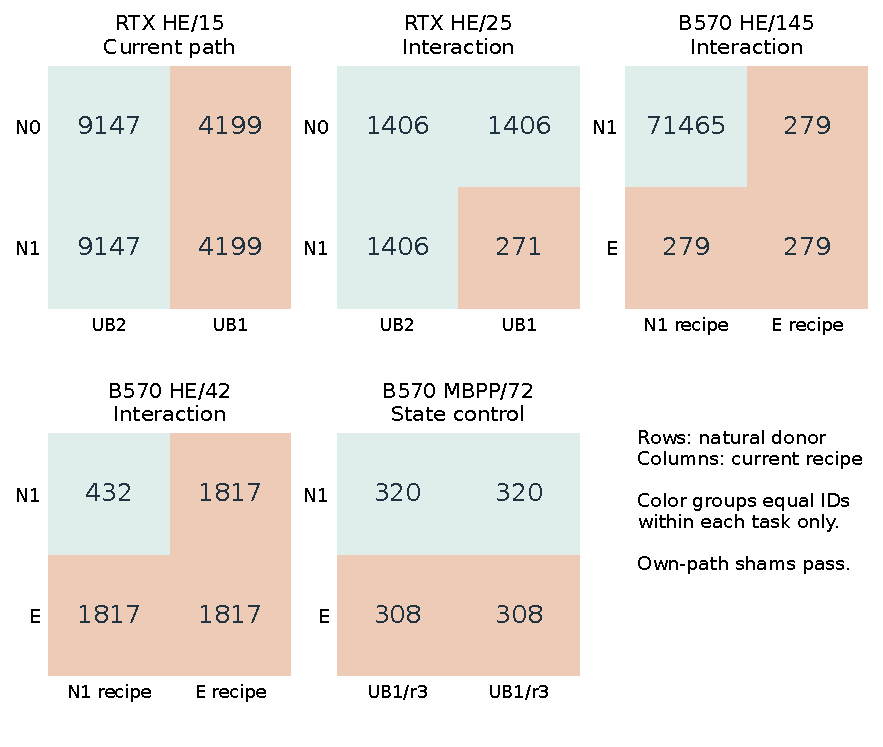
\includegraphics[width=\linewidth]{figures/figure_2_natural_crosses.pdf}
\caption{Source-derived RTX and B570 natural-state crosses. Rows are donors and columns current recipes. Cell labels are the discriminating sampled/argmax ID; colors group equal IDs within each task only. RTX /15 shows a current-path effect and /25 an interaction. B570 /145 and /42 cross N1 (UB1/reservation3) with E (UB2/reservation2); /72 has identical UB1/reservation3 current columns and is a state control. All repetitions reproduce the displayed local patterns.}
\label{fig:cross}
\end{figure}

The RTX donor comparison also distinguishes logical tensor equality from file hashes. All 12 prompt-KV pair comparisons agree, while 70 of 72 generated-prefix K/V tensor comparisons differ; tested first-layer logical K/V remain equal. This supports examining state formation and attention-related execution, but does not identify attention as the sole cause. In particular, the discriminating /15 bonus row is itself a single-token microbatch under both histories. The final row's nominal shape cannot explain the entire effect without considering its inputs and preceding work.

\subsection{One unchanged block does not certify the remaining trajectory}
A separate B570 experiment starts both branches from the same live fork state, with byte-checked KV, and intervenes on one target verification block, comparing UB1 with UB128. The frozen checkpoint is the first eligible block reached after at least 64 committed IDs. Twenty-four reserved prompts with three repetitions provide 72 eligible forks. All 72 paired raw score records change, yet top-1 IDs and actual immediate decisions do not: zero of 72 executions and zero of 24 tasks show an immediate decision difference across 195 paired decision events.

Continuing under the frozen policy gives a different result. Complete downstream committed-ID trajectories change in 18 of 72 executions, corresponding to six of 24 tasks. Later alternate target blocks retain UB128 and proposals evolve, so the secondary result is not an isolated one-block perturbation followed by restored execution. The score effect and delayed trajectory effect coexist with an immediate discrete null. The intervention's primary sampled-block result therefore cannot be relabeled either an immediate decision effect or a whole-output no-effect result. Its engineering implication is direct: qualification must continue beyond a locally unchanged acceptance decision. Neither logit movement nor one-step agreement replaces complete registered-output checking.

\subsection{B570 crosses identify a whole-recipe boundary}
Later B570 natural-state crosses cover three tasks in two contexts, with 12 complete own-path shams and 24 auxiliary target cells. Restored states are checked for byte consistency, sequence-zero ownership and logical position. Figure~\ref{fig:cross} includes the selected argmax matrices. HumanEval/145 has $[(71465,279),(279,279)]$ at prefix 56, and /42 has $[(432,1817),(1817,1817)]$ at prefix 73. Both are local interactions. MBPP/72 has $[(320,320),(308,308)]$ at prefix 40: donor state changes the decision while the current columns are the same UB1/output-reservation-3 recipe.

For the HumanEval crosses, the current recipes change microbatch and output reservation together. The appropriate causal factor is the current whole recipe, not UB alone. The repeated cases are three tasks, not six independent task discoveries. Full counterfactual continuations from each cross cell are unavailable; the subsequent candidate has a separate native endpoint qualification panel. The greedy sampler contract is supported by live history, clone metadata and shams, while opaque sampler bytes and general stochastic-state restoration remain unavailable.

These observations carry the same experimental question across CUDA and Vulkan without transferring the same repair. Some boundaries are path-sensitive, others state-sensitive or interactive. A runtime designer cannot infer the required control placement from committed-prefix equality or a single margin alone.

\subsection{Prediction and simple execution constrain added machinery}
Earlier prediction studies remain useful but answer a narrower question. B570 prospective prediction matches 72/72 native arrays on a reserved 24-task cohort even when reference agreement is 60/72. RTX's first target-only batched-path predictor reaches 24/36, below its frozen 36/36 gate, so that study performs zero reserved inference. A later independent-proposal replay implementation obtains H2/native and reference-only/native prediction agreement of 72/72, with reference agreement still 60/72. The first implementation's missing interface is resolved by that later study; neither result makes replay a cheap online repair.

A fresh ordinary target-only bridge provides an especially strong simple alternative. On the 19 RTX tasks, draft-free $U_2$ reproduces all 57 intervention $N_1$ arrays and strict stop boundaries without a draft, transplant, proposal tape or answer. It reproduces both /15's repair and /25's regression. This is output equivalence, not demonstrated equivalence of unavailable live logits/KV or a speed result.

Finally, retrospective selector feasibility finds no additional supported capability: RTX direct enumeration and proxy screening both abstain at 114 post-common-acquisition record equivalents; B570 needs 72 for direct verification and 144 for proxy screening. Unknown counterfactuals remain unknown. These costs are acquisition equivalents, not measured latency. Together, the results answer RQ1 with local state/path evidence while rejecting the shortcut from an accurate reproducer to a useful automatic repair selector.

\section{Phase-Scoped Implementation and Qualification (RQ2)}
\label{sec:repair}
\subsection{Constraining attention while retaining batched work}
The RTX candidate changes the non-flash Qwen3 attention subgraph inside \texttt{build\_attn\_mha}. An initial implementation constructs one attention subgraph per query and concatenates the results. A subsequent implementation represents query columns in the ggml batch dimension, allowing existing operations to process them in parallel while retaining a one-column query structure. Projection, output projection and feed-forward computation remain batched. The change is local to the graph representation, rather than global UB1 execution of every operation.

After the existing query/key/value permutations, the query tensor has dimensions $(d,q,h,1)$ in the supported single-KV-stream case. The candidate uses \texttt{ggml\_view\_4d} to reinterpret it as $(d,1,h,q)$, preserving the source strides and using the original query-column stride for the new batch axis. The attention mask similarly changes from a query-column layout to $(n_{\mathrm{KV}},1,1,q)$. Existing key-query multiplication, softmax, value multiplication and final contiguous recombination remain in the non-flash graph. Shared K/V tensors are not reconstructed from a reference answer. The purpose is to retain the tested scalar-query computation structure while preserving parallel execution elsewhere.

The source explicitly restricts this branch to Qwen3, non-flash attention, one KV stream, compatible mask dimensions, and absent attention bias, sinks and MLA value projection. The initial query limit is four; a source-bound later width build raises that assertion to eight without changing backend arithmetic. These guards define the implemented family. They do not establish invariance for every model graph, precision, shape or backend. Native output qualification supplies the behavioral evidence.

\subsection{Phase dispatch and graph reuse are part of the implementation}
The scope mask is process-fixed. A thread-local guard selects one of four bits by model role and by whether the call is prefill or continuation: target bits 1/2 and draft bits 4/8. It restores the prior active state on exit. The guard executes before the capture-disabled fast path returns to native \texttt{llama\_decode}, so disabling diagnostic metadata does not disable the constraint.

The selected boolean is copied into graph parameters and graph context. Graph reuse is rejected when that boolean differs from the cached topology key. This prevents a graph constructed for one phase layout from being reused solely because the ordinary microbatch fields match. The server also resets the phase to prefill when starting a new prompt. Scope selection is therefore an actual dispatch and reuse condition, rather than a label attached after execution.

Capture-disabled costs bypass observer metadata construction and forced observer synchronization. Qualification separately checks captured multi-query nodes and capture-on/off behavior. The source also contains a conditional target-state move after the first pending sample; the expansion environment does not set its activating continuation-UB variable. The measured RTX candidate consequently pays for native drafting, verification and reconciliation, but no state transplant is inferred merely from the presence of that branch. S1 and S2 bind the relevant patch files and timer audit.

\subsection{The finite phase family}
Figure~\ref{fig:phase} presents the full four-switch factorial: 16 masks, four exposed HumanEval probes and two repetitions, totaling 128 requests. All outputs and registered stop boundaries are repeat-stable. Masks 3, 7, 11 and 15 pass the complete probe panel. /15 and /31 pass every mask; /25 needs at least one target-phase bit; /18 needs both target phases. Draft-phase bits do not change this pattern.

\begin{figure}[!htbp]
\centering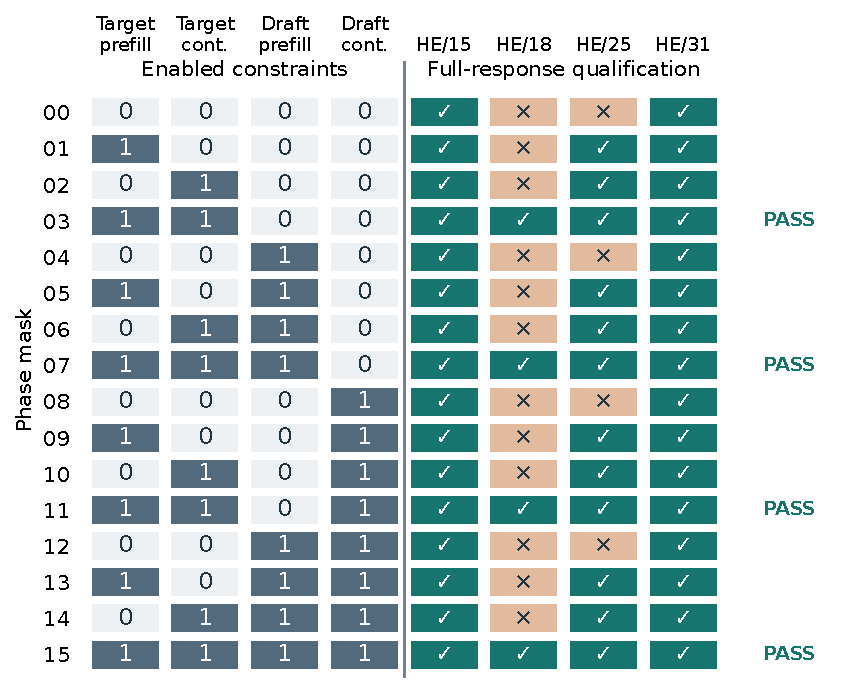
\includegraphics[width=\linewidth]{figures/figure_3_phase_matrix.pdf}
\caption{RTX phase qualification at fixed $k=3$, UB4 and cap128. Left columns show enabled phase bits; right columns show native full-response qualification for each probe in both repetitions. Passing masks are 3/7/11/15. Mask 3 is inclusion-minimal within this switch family; it is not an operator-level or all-input minimality theorem.}
\label{fig:phase}
\end{figure}

Mask 3 is the only passing set with no passing strict subset. This is inclusion-minimality in the registered family. The result neither proves that attention is the unique cause nor that draft behavior can be arbitrary in a different implementation. Acceptance, cache ownership, committed state and stopping still have to be valid. The $k=3$/UB4 factorial also differs from the original UB2/UB1 intervention, so /15's all-mask agreement does not erase its earlier path effect.

Scope is selected by qualification, not the fastest measured time. A subsequent 19-task, six-repetition cost panel gives mask 3 $1.278076\times$ generation and $1.112977\times$ request speed against matched target-only execution. Compared with mask 15, removing draft constraints adds only $1.003569\times$ generation speed, with descriptive interval $[0.997739,1.009456]$. It misses the frozen $1.03\times$ extra-generation gate. Fewer constrained phases do not automatically improve speed. The later 24-input expansion similarly gives only $1.015426\times$ extra generation benefit over mask 15.

\subsection{Frozen inputs and geometry boundaries}
The frozen mask-3/$k=3$/UB4 recipe qualifies all 96 candidate responses on the 24-input expansion in Section~\ref{sec:methods}. Matched target-only and mask-15 speculation also qualify. This extends sufficiency from exposed probes to a separately frozen input panel, while retaining the same model family and registered configuration.

Changing geometry exposes a failure boundary. An 11-input width/length panel separately tests $(k,\mathrm{UB})=(1,2),(3,4),(5,6),(7,8)$ at caps 128/256/512 with fresh scalar references. The first two pairs qualify. MBPP/229 fails at both wider pairs across caps and repetitions, while its matched controls pass. A separate old /18 geometry probe also fails at wider target-only capacity and remains outside the 11-task denominator. Actual long reference lengths reach at most 261; a cap of 512 does not demonstrate a full 512-token trajectory.

At MBPP/229's common 47-token prefix, naturally retained constrained and ordinary states are crossed under two UB6 query layouts. Four own-path shams reproduce their decisions. Donor state changes the EOG decision under either layout; the current layout changes continuous values without a separate discrete flip in these cells. Two cap contexts repeat one task boundary. This supports a local retained-state effect and shows why switching only the current layout there is insufficient. It does not identify a unique cause of every width failure.

\subsection{A separate B570 implementation and qualification scope}
B570 provides a distinct repair case. Its candidate constructs target state with the ordinary-reference prompt caller and output reservation, samples pending state once, then changes continuation UB128 to UB1 in the same context and live sampler. A private API synchronizes, changes the capacity and requests scheduler reservation under a frozen context/batch/sequence contract. Instrumented checks compare serialized KV before and after binding; formal capture-off requests omit witness readbacks. The existing $k=2$, draft-UB1 accept/bonus/rollback loop remains.

The candidate qualifies 12 development requests, 112 requests on 56 exposed inputs, and 30 requests on 15 project-unused inputs under its endpoint contract. It removes the old second context and three state witness readbacks, but does not implement the RTX query-layout transformation. Earlier B570 repair had a local long-panel positive result yet failed MBPP/72 on a new-input panel and failed five UB2 candidates. Those outcomes remain in S1. The later phase-binding candidate addresses qualification within its own scope; Section~\ref{sec:cost} assesses whether that repair pays.

\section{Does the Qualified Design Pay? (RQ3)}
\label{sec:cost}
\subsection{RTX: deployment gain and speculative increment}
The RTX expansion measures four conditions in four balanced rounds. Ordinary $R$ uses mask 0/UB1 without draft; matched $M$ uses mask 3/UB4 without draft; candidate $C$ uses mask 3/UB4/$k=3$; the all-scope condition uses mask 15. Each round has four separate resident processes, each with one excluded warmup and 24 formal requests. Condition and task orders rotate; recorded cache reuse is zero. Thus the paths share a panel and campaign but not one simultaneous resident process.

Table~\ref{tab:rtx_cost} reports the same-record CPU reconstruction against both paid baselines. Generation speed is $1.170124\times$ ordinary and $1.169238\times$ matched execution, with 22/24 tasks faster in each comparison. Resident-request speed is $1.741569\times$ ordinary but $1.035071\times$ matched. Crucially, $R/M$ request speed is $1.682560\times$: most of the ordinary-reference request improvement is available without speculation. The $1.742\times$ result is the benefit of the full deployment change and cannot be assigned entirely to speculative execution.

% Generated by scripts/reconstruct.py from frozen exports.
\begin{table}[ht]\centering\small
\caption{RTX frozen expansion paid ratios: 24 task medians, four repeats. Intervals describe task resampling. $C_3$ is mask 3 speculation.}\label{tab:rtx_cost}
\begin{tabular}{@{}lrrrr@{}}\toprule
Ratio & Gen. & Interval & Request & Interval\\\midrule
$R$/$C_3$ & 1.170124 & [1.117,1.218] & 1.741569 & [1.655,1.827]\\
$M$/$C_3$ & 1.169238 & [1.117,1.217] & 1.035071 & [1.005,1.063]\\
$R$/$M$ & 1.000758 & [0.995,1.008] & 1.682560 & [1.590,1.766]\\
\bottomrule\end{tabular}

\end{table}


Figure~\ref{fig:cost} displays the three comparisons on a common baseline/candidate axis while keeping generation and resident-request intervals distinct. Equation~\ref{eq:identity} is verified for all 48 task-level timer identities and both aggregate identities. This consistency check explains why the three ratios fit together; it does not measure which component contributes a fraction of the saving.

\begin{figure}[!htbp]
\centering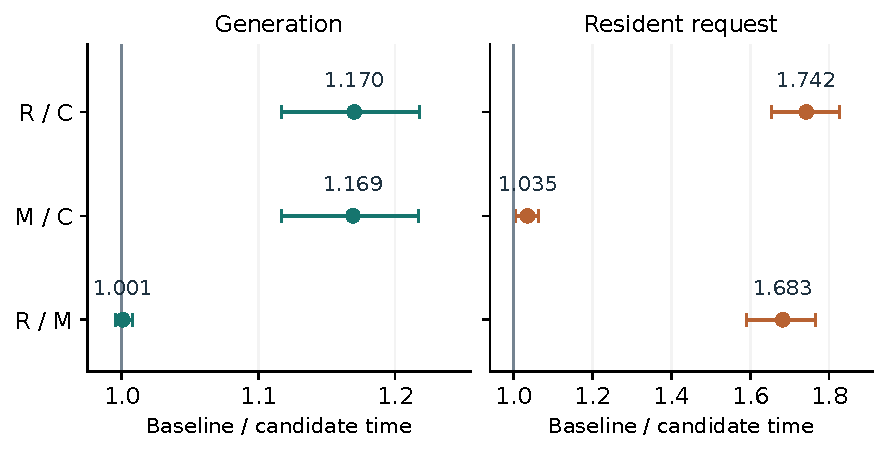
\includegraphics[width=\linewidth]{figures/figure_4_paid_cost.pdf}
\caption{RTX expansion paid speed ratios with descriptive task-bootstrap intervals. Ordinary/candidate measures the deployment change; matched/candidate the increment from speculation; ordinary/matched the draft-free path change. The two timers cover different intervals. Ratios are not additive component costs.}
\label{fig:cost}
\end{figure}

The target-path comparison changes prefill microbatch/attention behavior and continuation capacity jointly. Generation $R/M$ is near parity, whereas the request ratio is much larger. Without independent profiling, that contrast cannot quantify attention, KV, transport, synchronization or host shares. It also cannot certify that $R$ is the fastest ordinary decoder. A faster qualified ordinary implementation could narrow the deployment benefit without changing the arithmetic reported here.

\subsection{Task variation and session uncertainty}
The incremental request benefit is modest and uneven. Figure~\ref{fig:tasks} keeps task generation and request ratios in the same request-sorted order. Seven tasks are slower than matched execution, although all 24 are faster than ordinary request cost. Matched-request round 2 reverses direction at $0.940220\times$; the other round geometric means are approximately 1.029, 1.052 and 1.044. The descriptive task interval for the median-based aggregate lies above one, but does not erase that reversal.

\begin{figure}[!htbp]
\centering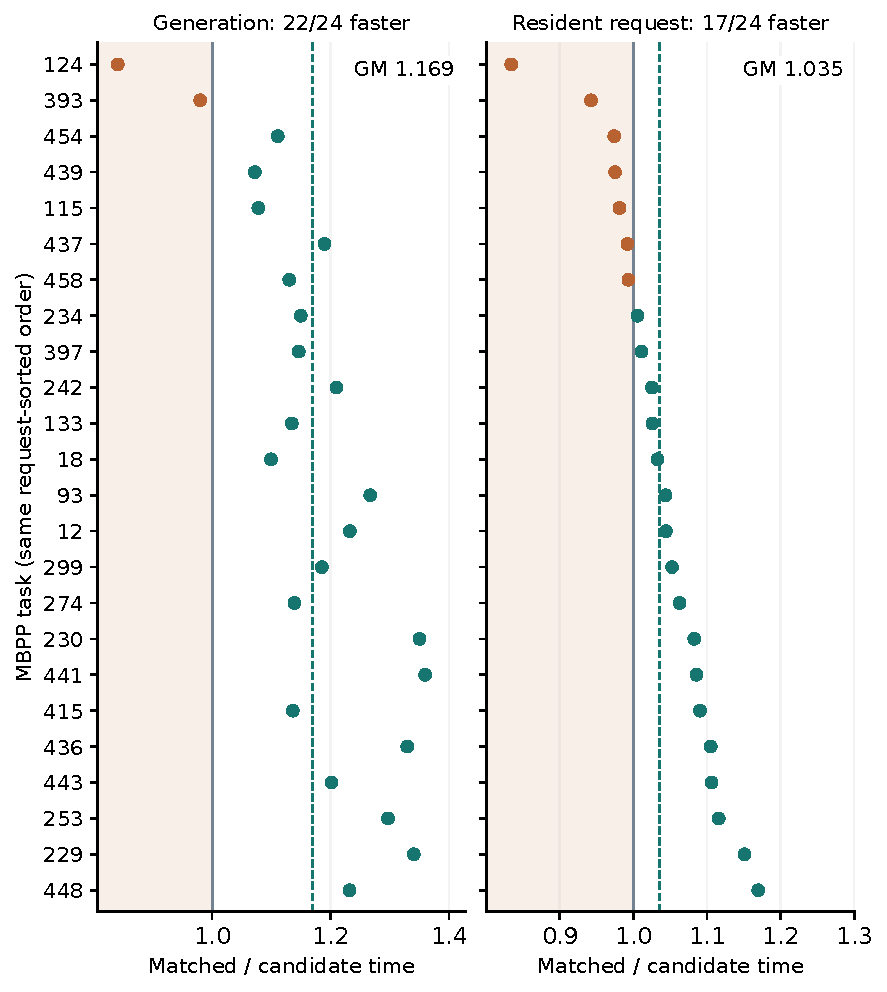
\includegraphics[width=\linewidth]{figures/figure_5_task_variation.pdf}
\caption{RTX matched/candidate task ratios from four-repetition absolute-time medians, in a shared order sorted by request ratio. Points represent tasks. Generation improves on 22/24 and resident request on 17/24; seven request regressions remain. Dashed lines mark aggregate geometric means and the solid parity line marks one.}
\label{fig:tasks}
\end{figure}

Separate resident sessions, laptop scheduling and thermal variation can affect these estimates. Balanced order and task medians reveal some variation but do not remove session confounding. A task bootstrap is not independent session/day replication. We therefore report a qualified positive aggregate operating point, rather than stable production request acceleration. The larger generation gain remains a result for its defined interval, not an end-to-end substitute.

The serial resident-reset study supplies a separate finite check: recorded requests begin with reset target state and the original $k=3$/UB4 recipe retains reference output across two request orders. Its matched generation/request speeds are about $1.181\times/1.039\times$. This supports the registered reset behavior. It is not a concurrency or throughput experiment and is not pooled with the 384 expansion rows.

\subsection{Fixed UB: wider drafting qualifies but becomes slower}
The geometry failures in Section~\ref{sec:repair} change $k$ and UB together. A separate frozen experiment holds UB4 and mask 3 fixed while testing $k=3,5,7$ on 24 now-exposed MBPP inputs plus four exposed HumanEval probes. All widths qualify in two repetitions. The highest passing $k=7$ is selected by qualification alone, then measured in separate capture-off sessions: four conditions, four repetitions and 448 formal requests. Qualification timings are excluded from speed selection.

Relative to the $k=3$ anchor, $k=7$ reaches only $0.829442\times$ generation and $0.889868\times$ resident-request speed. Against matched target-only, it reaches $0.997404\times/0.950353\times$, while the anchor reaches $1.202501\times/1.067970\times$ in that campaign. The widened candidate preserves the reference and fails the extra-cost objective. Ordinary same-width speculation has output failures, so its times remain diagnostic rather than qualified speed evidence.

Formal draft work grows from 3,528 to 5,392 tokens while accepted draft tokens grow from 2,772 to 3,192. In separate captured qualification sessions, target continuation caller calls fall from 305 to 199, but observed micrographs rise from 305 to 397. These sessions include their own warmups and forced synchronization; the counts cannot be combined with formal times into a fabricated per-call profile. Micrographs are not CUDA kernel launches. The evidence rejects caller reduction as a sufficient performance proxy without assigning the slowdown to a unique component.

Saved partitions also matter. At $k=7$, matched generation/request speed is $0.953/0.919\times$ on 24 MBPP inputs but $1.308/1.164\times$ on four HumanEval probes. The pooled result hides these differences. Four exposed probes do not validate a routing rule, and no online selector was developed from them. S1 retains the longer-cap confirmation and the failed wider-geometry branches without combining their timers into an optimization trajectory.

\subsection{B570: repair improves an old path but loses to strong baselines}
The B570 formal matrix remains 119/120 complete: old N1's first-round MBPP/400 payload is missing after an infrastructure interruption. No request is imputed or rerun in the scientific denominator. Ordinary $R$, matched $M$ and candidate $C$ each have 30 complete responses, providing 15 two-round task-median pairs. Old-N1 comparisons have 14 complete task pairs.

Table~\ref{tab:b570_cost} gives all three timers. Candidate speed is $0.282588\times$ generation and $0.201290\times$ whole request against ordinary $R$, and $0.285761\times/0.205704\times$ against matched target-only. Both baselines are faster in every available paired round. The matched target path is close to ordinary cost ($R/M=0.988893\times/0.978539\times$), so the roughly fivefold candidate request cost cannot be attributed entirely to the consistency constraint on the target path.

% Generated by scripts/reconstruct.py from frozen exports.
\begin{table}[ht]\centering\small
\caption{B570 paid baseline/candidate task-median ratios. Complete two-round pairs only; the missing old-N1 task is not imputed. All raw suffix work stays charged.}\label{tab:b570_cost}
\begin{tabular}{@{}lrrrr@{}}\toprule
Ratio & Tasks & Generation & Whole request & Host\\\midrule
$R/C$ & 15 & 0.282588 & 0.201290 & 0.201884\\
$M/C$ & 15 & 0.285761 & 0.205704 & 0.206243\\
Old N1/$C$ & 14 & 3.993091 & 2.633940 & 2.633387\\
$R/M$ & 15 & 0.988893 & 0.978539 & 0.978864\\
\bottomrule\end{tabular}

\end{table}


Against old N1, the candidate improves generation/request speed by $3.993091\times/2.633940\times$ over 14 task pairs. That is real engineering progress relative to a slow prior frontend, but does not establish deployment benefit. MBPP/245 also reverses the old-path request comparison in round 2. Neither aggregate improvement nor endpoint recovery supports a universal per-round gain.

The candidate's formal records contain 888 drafted and 702 accepted tokens. Endpoint IDs total 1,150 while raw IDs total 1,176; all 26 suffix IDs remain charged. Target and draft continuation caller-token totals are 1,332 and 1,362. These are distinct runtime quantities. Raw suffix equality is not required by this endpoint contract and is not claimed. Removing witness readbacks, an extra context and handoff improves the frontend, while phase reservation, synchronization, drafting and rollback remain online. No full independent component profile identifies a unique remaining bottleneck. The appropriate decision is to reject this recipe as a latency improvement against the two strong baselines.

\subsection{Global serialization, control, and draft-side limits}
An earlier RTX global-serialization timing arm qualifies 57/57 arrays on 19 exposed tasks but reaches only $0.677351\times$ target-only speed, with descriptive interval approximately $[0.662,0.692]$ and zero tasks faster. Its synchronized post-prefill-to-slot-release interval includes instrumented work and logging, unlike the later server generation field. It is a separate qualified cost failure, not the first point of a common before/after speed curve. S1 preserves its host-timer amendment and the preceding V3 stop.

M4 provides a contrasting control decision under its own contract. A prospective 60-task, three-condition, three-repeat campaign has 540 requests; both fixed Always speculation and Guard qualify 180/180 direct generated-ID comparisons. Against target-only, their post-prefill speeds are $1.346894\times$ and $1.311387\times$. A paired secondary analysis gives Guard/Always latency $1.027076$, with descriptive interval $[1.012956,1.043559]$: this guard is slower on the measured comparison. It should not be retained on the premise that adaptivity necessarily improves performance.

A hindsight per-task oracle choosing only target-only or Always leaves about 0.069\% further geometric-mean latency reduction relative to Always. This is a panel-specific two-action opportunity, not an upper bound on intra-request policies. HumanEval and Spec-Bench fixed-policy speeds also differ ($1.570\times$ versus $1.155\times$). The formal direct-ID study is distinct from earlier M4 text-based and proxy measurements.

On 358H, CPU/NPU drafting each qualifies its 90-request direct-ID panel but yields $0.733915\times/0.351663\times$ speed. With baseline cost $B_{ij}$, measured target work $T_{ij}$ and progress fixed, removing all other nonnegative work gives the conditional budget
\begin{equation}
\operatorname{GM}_{i}\operatorname{median}_{j} S'_{ij}
\leq \operatorname{GM}_{i}\operatorname{median}_{j}(B_{ij}/T_{ij}).
\label{eq:floor}
\end{equation}
Prompt-estimator ceilings are $0.8372\times/0.8448\times$, still below parity. Even deleting all other work would require a uniform target-work reduction of at least 16.28\%/15.52\% to reach parity under that estimator. Pooled-total ceilings differ and remain in S1. Full-prefix NPU replay is an implementation cost, not a theorem against heterogeneous inference. This case redirects optimization toward target work or a different state interface; faster isolated drafting alone cannot meet the measured budget.

\section{Design Implications and Limits}
\label{sec:implications}
\subsection{Constrain the transaction where evidence warrants it}
The useful outcome of diagnosis is a smaller design space. A current-path effect motivates controlling verification geometry; a retained-state effect requires preserving the state-producing path or changing its interface; an interaction requires checking both. The RTX crosses justify testing a local attention layout with target-phase switches. The B570 crosses motivate phase binding within one context and expose why changing only current reservation cannot repair a state-dependent case. Neither observation uniquely identifies a kernel, and neither turns the diagnostic procedure into an automatic selector.

These distinctions also determine what must be tested after a change. A successful immediate argmax check leaves downstream state unconstrained. A passing natural cross verifies one aligned cut, not the complete response. The single-block B570 result demonstrates the gap directly. Complete output qualification therefore follows local diagnosis and precedes any speed claim. The endpoint contract must be chosen before evaluation: discarding post-EOG IDs for B570 comparison is legitimate under its registered contract, but all paid suffix work stays in cost.

Locality is a property of this implementation rather than a synonym for low overhead. The RTX transformation retains batched projections and FFN while reshaping attention queries, and its phase switches restrict which transactions use that graph. Mask 3 needs fewer constrained phases than mask 15 to qualify the tested probes, yet the registered extra generation-speed gate is not met. Fewer constrained stages may simplify a design or reduce its exposure to numerical changes without creating a measurable speed improvement.

\subsection{Use the matched path to decide whether to add a draft}
An ordinary comparison answers whether replacing a deployed reference path helps. A matched comparison answers whether the proposed speculative transaction helps beyond its draft-free target path. Both are engineering questions. Reporting only ordinary RTX request speed would hide that most of the measured improvement comes from a qualified target-path change. Reporting only the matched result would hide the measured deployment opportunity. The ordinary reference remains a paid, qualified comparator; its role does not imply optimal ordinary decoding.

The counterexamples change concrete decisions. On the frozen RTX operating point, speculation adds generation benefit and a small aggregate request benefit, with seven task regressions and a reversed round. The fixed-UB widened draft should not replace that anchor for latency on the pooled panel. The B570 repaired candidate should not replace either strong baseline despite outperforming old N1. On M4, the measured guard should not be added to the fixed policy on an assumed control benefit. On 358H, draft-only work cannot remove the measured target-work deficit under the stated fixed-progress budget. These are configuration-specific decisions, not a platform ranking.

\subsection{Scope of the evidence}
The repair study uses one target/draft model family, Qwen3, with finite prompt panels and pinned runtime variants. It establishes neither cross-family transfer nor lossless behavior on arbitrary inputs. The RTX project-unused panel limits prior project exposure but is still a selected 24-input MBPP panel. Wider geometry failures show that configuration changes require renewed qualification. A second model-family study can be inserted after the phase qualification and before the paid-cost comparison, with its own frozen configuration and endpoints; this manuscript contains no expected results for that extension.

Greedy argmax is discrete and can expose small numerical differences near a decision boundary. The observed score and KV differences do not separate all reduction, precision, layout and scheduling effects. Full-response agreement is an empirical gate, not a proof of numerical equivalence. Natural donor states and own-path shams strengthen the local intervention interpretation but cannot exhaust hidden backend state or establish a universal minimal repair.

Task medians and descriptive intervals summarize the saved campaigns. They do not eliminate repeated-session, thermal, ordering or infrastructure effects. B570's missing old-N1 row and unknown raw comparisons remain explicit. Historical timing and energy domains differ; stronger later qualification cannot retroactively certify earlier timings. The author-side CPU verification checks the committed exports and source bindings, not every private raw archive, an external peer review or a commercial similarity assessment. S1 and S2 identify the inspected material and the remaining author obligations.

\section{Conclusion}
Reference-preserving speculative execution requires a qualified transaction, not merely correct acceptance logic at one decision. The studied RTX implementation constrains attention query layout during target prefill and continuation while retaining other batched computation. Natural crosses and a four-switch qualification study support that finite repair scope; complete responses and width failures define its boundary. Paid ordinary and matched comparisons then separate the deployment gain from the speculative increment. The resulting decisions are mixed: the frozen RTX anchor helps on aggregate, a wider qualified draft loses, the B570 repair remains slower than strong baselines, and M4 and 358H restrict the case for added control and draft-only optimization. The study supplies concrete implementation evidence and reproducible cost comparisons within one model family, while preserving failures that prevent broader claims.

\section*{Author-review declarations}
\textbf{Authorship and contributions.} Author names, affiliations, corresponding-author details and individual CRediT roles await author confirmation. This draft does not assign authorship or contributions.

\textbf{Funding and competing interests.} Funding sources and competing-interest declarations await confirmation by all authors; absence of a funding source or competing interest is not asserted.

\textbf{Data and software availability.} The author-review source package includes frozen committed evidence exports, source bindings, selected implementation and report records, and CPU-only code for recalculation and figures. Original runtime code and experiment records are retained in the HeteroSpec project. Availability and permitted redistribution of private raw archives, model artifacts and a permanent public data/software location require author confirmation before submission. The supplied exports enable the numerical checks specified in S1; they do not substitute for a full private-archive audit or a rerun of model inference.

\textbf{Declaration of generative AI and AI-assisted technologies in manuscript preparation.} OpenAI ChatGPT/Codex was used to assist with restructuring and drafting text, source and bibliography checks, CPU analysis and plotting code, and the execution-architecture illustration. Quantitative figures are generated from the identified experimental exports, without generative replacement of observations. This author-review version still requires the authors' final scientific, bibliographic and language verification. The final declaration and responsibility statement must be confirmed by the authors before submission.

\begingroup\small
\bibliographystyle{elsarticle-num}
\bibliography{references}
\endgroup
\end{document}
